% Chapter 2

\chapter{Personal transport, energy and commuting}
\label{Chapter2}
\lhead{Chapter 2. \emph{Personal transport, energy and commuting}}
% \lhead{Chapter 2. \emph{Commuting and its energy implications}} %
% \lhead{Chapter 2. \emph{The Energy Costs of Transport: A Review}}
\fancyhead[RO,LE]{Chapter 2. Personal transport, energy and commuting} %2side
\fancyhead[RE,LO]{\thepage}
%%% Really happy with this introductory text: reads nicely.
%%% Could I write this as a paper? May be worth it...

\begin{quote}
\textit{The traditional preoccupation with the supply side of transport policy
---
the provision of additional road, air and rail infrastructures --- is no longer
appropriate socially, economically and environmentally.}
\flushright{\citep[p.~5]{Peake1994}}
\end{quote}

Any review of research into the energy consumption of commuters is bound to
encounter wider issues such as transport infrastructure,
% --- which once in
% place, can affect transport flows for decades \citep{Whitelegg1987} ---
the spatial characteristics of labour markets \citep{Ballas2006}, population
densities of settlements \citep{Breheny1995}
and the price of oil \citep{Sexton2011}. Transport research is often
multidisciplinary \citep{Hoyle1992modern}. This element is even more important in
the present study because
commuting and energy use in transport are not academic disciplines, or even
established fields, of their own right. Rather they are issues, tackled from a
range of perspectives using various methods. 

As illustrated by the quote that opens this chapter,
research into energy in transport is
contested. Almost 20 years since it was written
there has undoubtedly been much more focus on the demand side;
social and environmental considerations have increasingly been
taken into account; and transport studies have become more
multi-disciplinary. Yet fundamental differences in the methods used by
researchers persist. Battle lines can be seen emerging in the literature,
for example, between those
who advocate a greater role for the social sciences \citep{Schwanen2011} and
those who advocate a scientific approach 
\citep{Simini2012, Marshall2008}. The transport-energy nexus has also received
attention from disciplines not traditionally associated with either issue,
such as computer science, physics and psychology.  It is therefore necessary to
impose some kind of order on the mass of work that is related to the topic.
With this aim in mind, the literature reviewed is divided into six sections:
\begin{itemize}
 \item the `sustainable mobility' paradigm (\cref{ssus})
 \item commuting research, at various scales   (\cref{s:commuting})
 \item energy use and emissions in personal transport generally (\cref{s:energy})
 \item energy impacts of commuting specifically (\cref{sdisciplines})
\item `tools of the trade' --- methods for studying energy and commuting
(\cref{s:tools})
\item key concepts in energy and commuting (\cref{skeyconcepts})
\end{itemize}
These sections initially deal with commuting and
transport energy use as separate entities,
because they have rarely overlapped. The studies that
do tackle the interface between these issues are generally conducted from
within pre-existing disciplines, such as economics or transport geography,
rather than adopting a completely multidisciplinary approach or attempting
to start a new field in `transport and energy', let alone
`energy use in commuting studies'.
\Cref{sdisciplines} therefore focuses on two studies
that deal with energy and commuting from two different perspectives:
transport geography and economics.
% have most to say in this
% regard, but drawing disciplinary boundaries in the field is probably
% not useful, so the section is structured by the research focus
% (life-cycle analysis, energy use of different modes etc.).
Because this
research area is quite specific, the section is the only one in which
comprehensive coverage is attempted. The other sections attempt
only to outline influential strands of research and highlight findings
of direct relevance to this project. \Cref{s:tools} provides
an overview of the techniques used in the research areas covered, and introduces
one of the main methods: spatial microsimulation.
(The spatial microsimulation literature is covered in more detail in
\cref{Chapter3}.)
The current chapter
concludes with a summary of important knowledge gaps in the area of
commuter energy costs, and promising research directions that
are related to the thesis (\cref{sc2sum}).
%%% This where we've hit the end (the section is only 1 paragraph long - Jan 2013)
%%% Ideally each section should be ~2,000 words long (10,000 / 4), less with images.

\section{The sustainable mobility paradigm} \label{ssus}
As outlined in \cref{Chapter1}, energy use in transport is bound-up with a
number of issues --- climate change, energy, inequality.
Diverse as these are, they all fall within
the umbrella term of sustainability. It is not surprising, therefore, that much
of the work linking transport and energy use has been conducted within the context of
sustainability, especially since the 1990s when sustainability became a buzzword
in politics and academia. Here is not the place to discuss
of what sustainability does and does not mean.\footnote{See \citep{Pezzey1997} for an
attempt to define the term rigorously or \citep{Steg2005} for a discussion
of `sustainable transportation'.
}
For the purposes of this section, suffice to
say that sustainability relates to \emph{long-term} environmental, social and
economic well-being. According to \citet{Banister2008}, in a paper with the
same title as this section, sustainable mobility is an approach to transport
research and policy that differs from conventional transport planning priorities
in the following ways:
\begin{itemize}
 \item its focus on people and social outcomes rather than infrastructure,
 vehicles and traffic
 \item localised and specific in its approach to intervention, rather than large
 scale and homogeneous
 \item a focus on potential scenarios of the future rather than univariate `modelling'
 \item travel modes placed in a hierarchy with pedestrians and cyclists at the top,
 rather than a focus on motorised transport
 \item multi-criteria assessment methods used for project assessment
 rather than just economic valuation
\end{itemize}
On all counts, the world-view adopted in this research project
fits firmly into the sustainable mobility
paradigm, so this is the starting point for the literature review. Energy use
in personal transport may seem a technical consideration, suitable for consideration
only by traffic engineers and natural resource economists. Yet the energy intensity
of transport systems has a direct impact on resource depletion (and therefore
economic sustainability), the natural environment and, by amplifying inequalities
in access to physical and cultural resources, people's lives.
The energy costs of commuting is therefore of critical importance to
the ability of modern economies to sustain themselves.

Probably the most high-profile UK government report written from the perspective
of the sustainable mobility was published by the Sustainable Development
Commission (SDC) \citep{Kay2011}.\footnote{This report, incidentally, was
published just before the SDC was dissolved
by the coalition government in March 2011. No follow-up research
in the area has been conducted.
}
`Fairness in a Car
Dependent Society' takes
a broad perspective when analysing personal transport.
As advocated by \citet{Banister2008},
it focuses on people rather than traffic and infrastructure, while also mentioning
the potential for environmental and (long-term) economic gain.
The report urges the prioritisation of
``quality of life, safety and the environment'' for all members of society
affected by personal travel systems over the speed and convenience of
wealthy travellers \citep[p.~5]{Kay2011}. The report's findings are
especially powerful because it provided a very large body of evidence
to support its findings, rather than to simply repeat the `anti-car' mantra
expounded by some based on the strength of rhetoric, social-theory and
a smattering of technical facts (e.g.~\citealp{Dennis2009}).
% An example of this insistence on evidence to support the argument
% is presented in \cref{fcrashnssec}: the simple visualisation
% vividly illustrates the problem in an politically neutral way, for
% maximum impact. Although traffic-related deaths and injuries are outside
% the scope of this PhD, the approach to quantitative evidence embodied in
% \cref{fcrashnssec} is something to which this thesis aspires.
% 
% \begin{figure}[htbp]
%   \centerline{
%     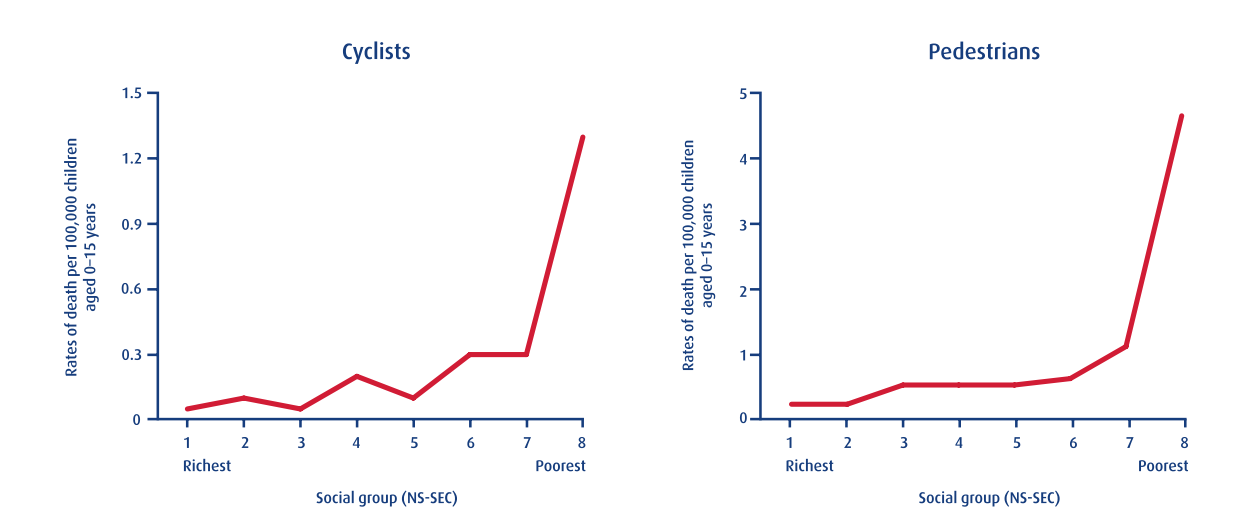
\includegraphics[width = 14 cm]{crashesnssec}}
%   \caption[The relationship between class and traffic-related deaths]
%   {The relationship between social class and traffic-related deaths
%   \citep{Kay2011}}
%   \label{fcrashnssec}
% \end{figure}

\citet{Kay2011} is also useful as a source of inspiration about
future interventions, as it provides %!!! mention kay in concs.
strong and specific policy recommendations. The most general of these, that 
can be applied to nearly every intervention affecting transport, is that a clear order
of priorities should be followed by transport policy-makers (\cref{fsdc}).
Incidentally, this is the same order of priorities that would be
followed if reducing energy use were the primary objective of
transport policy, as the evidence presented in chapter 1 suggests it should be.

This thesis is therefore closely related to the SDC study (and
the sustainable mobility paradigm more generally) in a number of ways.
It begins from the same world-view as \citet{Banister2008}, but
focuses on energy as a way to include all the various
factors affecting sustainability. The purpose of this research mirrors
that of \citet{Kay2011}:  to highlight the wider impacts of
personal mobility.
The methods are quite different, however: based \index{fairness}
on the knowledge that a range of social, economic and environmental ills are
associated with energy intensive transport highlighted in \cref{Chapter1}, the focus
is on
% not on the fairness and social outcomes favoured by \citet{Banister2008}
% and \citet{Kay2011}, but
energy use. This thesis does also
highlight the wider costs to society of personal travel advocated
in the `sustainable mobility paradigm', but indirectly,
via energy use, and with a focus on only one type of trip: commuting.

\begin{figure}[htbp]
  \centerline{
    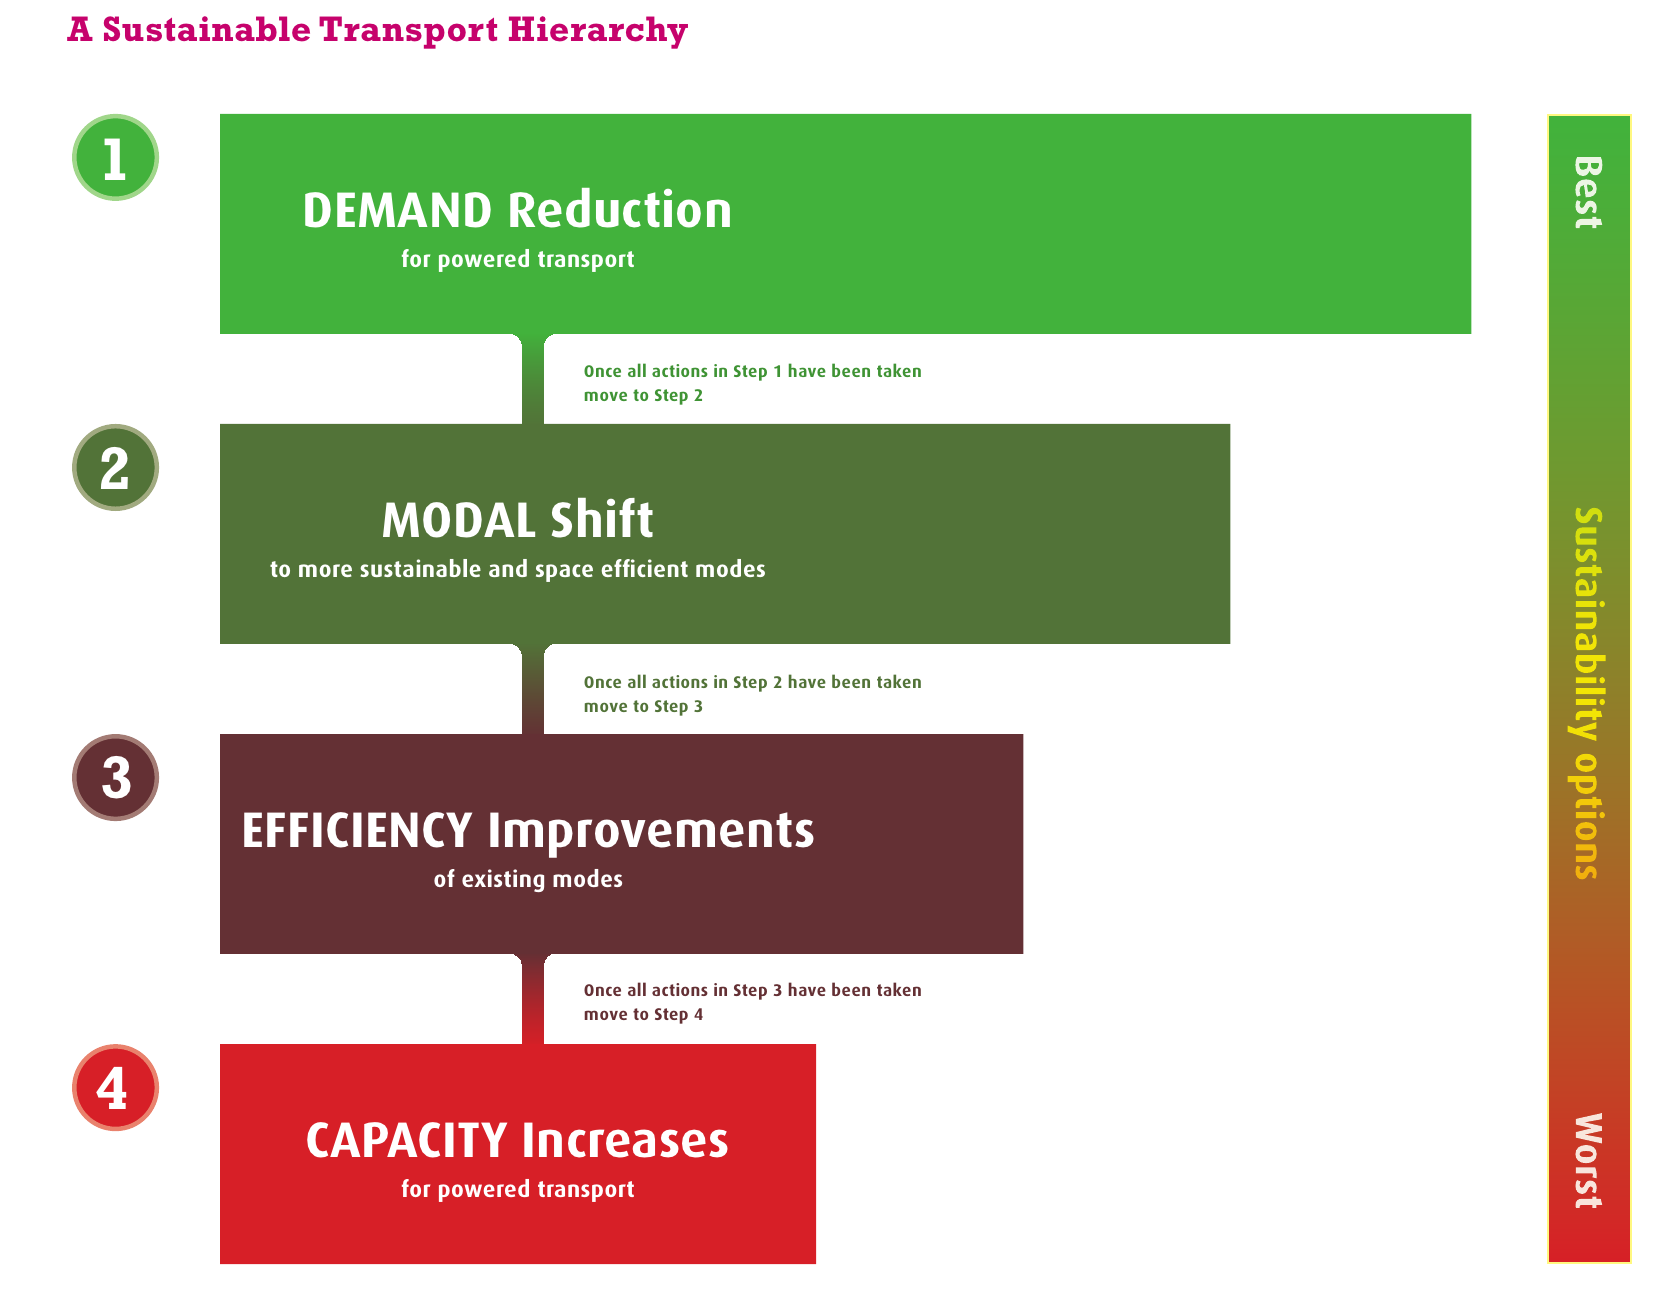
\includegraphics[width = 10 cm]{Sustainable-trans-hierarchy}}
  \caption{The sustainable transport hierarchy \citep{Kay2011}.} %%% could update with methods
  \label{fsdc}
\end{figure}

\subsection{Active travel} \label{sactive}
Although not always explicitly part of the sustainable mobility
paradigm, many of the studies from the loosely defined `active travel'
literature\footnote{This
area of
research has also been referred to `non-motorised transport', or simply
`walking and cycling'. The term `active travel' is preferred as it is more
concise and encapsulates all methods of travel to work that rely on human
muscles rather than mass-produced motors as prime-movers (see
\citealp{Smil2008} for more on the contrasts and surprising similarities between
the two). The rare but growing category of muscle-motor hybrid vehicles such as
electric bicycles is ambiguous is in this regard: as the ratio of motive energy
provided by personal exertion and inanimate energy sources will vary between
zero and infinity from case to case. The approach taken here is to exclude it
from active travel completely as motors and their energy supply must be
included for a realistic energy assessment.
%ref
}
make reference to the sustainability benefits of walking and cycling. For
the purposes of this literature review, research into non-motorised modes is
therefore considered as part of sustainable mobility,
although the term has been used in different
contexts.\footnote{Lawrence Burns, who directs the Program on Sustainable
Mobility at Columbia University's Earth Institute,
uses `sustainable mobility' primarily to describe shifts in
car technology and use, including driver-less cars and electrification \citet{Burns2013}.
\citet{Aftabuzzaman2011} uses the term to describe a transport system
resilient in the face of peak oil.
}
Much
of the active travel literature
has a clear health agenda (e.g.~\citealp{Jarrett2012}); here the focus is
on studies that also report energy and emissions implications.

\citet{Woodcock2007} investigated the links between transport, the environment
and health by projecting the rate of active travel up to 2030 in London.
The outcome of policies to encourage cycling were found to be wide ranging,
including positive impacts on road injury rates (a `neglected epidemic'), physical
inactivity and associated degenerative diseases, climate change and pollution,
`community severance', as well as difficult-to-measure impacts on energy
security and rates of transmission of infectious diseases. Clearly it is not
possible to accurately measure each of these impacts in a single study, but
it is useful to bear in mind the broader benefits of walking and cycling, which
are also particularly energy efficient. In a similar vein, \citet{Jacobsen2009}
provided evidence to suggest that as well as competing with healthier
and lower-energy active travel modes
for trips and space, motorised traffic also discourages walking and cycling
through perceived danger levels. Although their methodology was relatively
rudimentary (a review of statistics from the academic and policy literature),
\citet{Jacobsen2009} provide the basis for an interesting hypothesis:
that strategies to reduce
car use may be more effective than pro-active travel measures in terms of energy
and health outcomes. The case study comparing commuter energy use between
the UK and the Netherlands presented in \cref{sinternational} provides some
empirical support for this hypothesis.

With the emergence of newly available datasets from GPS devices, mobile phones
and bicycle rental schemes, more sophisticated methods have emerged in
the realm of active travel research. \citet{Ogil-cambridge2010}, for example,
provide details of how GPS measurements for individuals can be used
estimate both physical activity levels and CO$_2$ savings of active travel.
In-depth questionnaires were also used to estimate
``physical activity energy expenditure (PAEE) and total energy expenditure (TEE)''
\citep[p.~7]{Ogil-cambridge2010}. GPS data was combined with
accelerometer data by \citet{Cooper2010} to estimate physical activity. Although this
metabolic energy consumption of the human body is not
generally seen in the same light as energy use by vehicles, both can be measured
in the same units and compared directly. It is argued in \cref{Chapter5} that
this fact is a further benefit of the energy approach to commuting: substituting
motorised energy use with muscular energy has a direct impact on obesity and
chronic inactivity levels. Thus energy measurements can
encapsulate (to some degree) health as well as environmental impacts of travel.

In line with this new abundance of data, advances have been made in
characterising and 
modelling active travel patterns also. \citet{Millward2013} used GPS
data to supplement survey findings on walking trip characteristics in a US
city. The combination allowed for accurate characterisation of both
quantitative variables such as speed, time and distance of travel as well
as qualitative information about the reason for trip.
Of particular relevance to scenarios of
future change, is work looking at the `impedance functions' of active travel
modes with respect to distance under various conditions \citep{Iacono2010}.
Here, impedance refers to the disincentive to make trips by active travel per
unit distance.
Impedance influences $p$, the proportion trips that
take place between A and B made by walking or cycling. Due to the impedance or 
`resistance' to travel associated with these modes being highly dependent on distance
compared with faster and 
less physically demanding motorised modes, the proportion of trips made by them
can be expressed as a function of distance ($p = f(d)$). Based on this reasoning
$p$ should be high for the shortest
trips, dropping rapidly as the distance increases beyond a few kilometres
and leveling-off towards 0\%  after around 5 km for walking and 15 km for cycling. 
This hypothesis has indeed been born-out in practice.
Based on travel survey data, \citet{Iacono2010} calculated the rate
at which the proportion of trips made by bicycle and walking decreases
with increasing distance for different trip reasons, including shopping and
commuting \cref{fimpedance}.
The average proportion of trips ($p$) made by a particular mode in a particular context
(e.g.~bicycles for shopping in a given settlement) was found by \citet{Iacono2010}
to take the following functional form:
\index{impedance}
\begin{equation}
 p = \alpha \times e^{- \beta \times d}
 \label{eimpedance}
\end{equation}
where $\alpha$, the proportion of made for the shortest distances
and $\beta$, the rate of decay
are parameters to be calculated from empirical evidence. 
This equation is interpreted in \cref{Chapter8} as a proxy for the probability
of car-bicycle modal shift.


\begin{figure}[htbp]
  \centerline{
    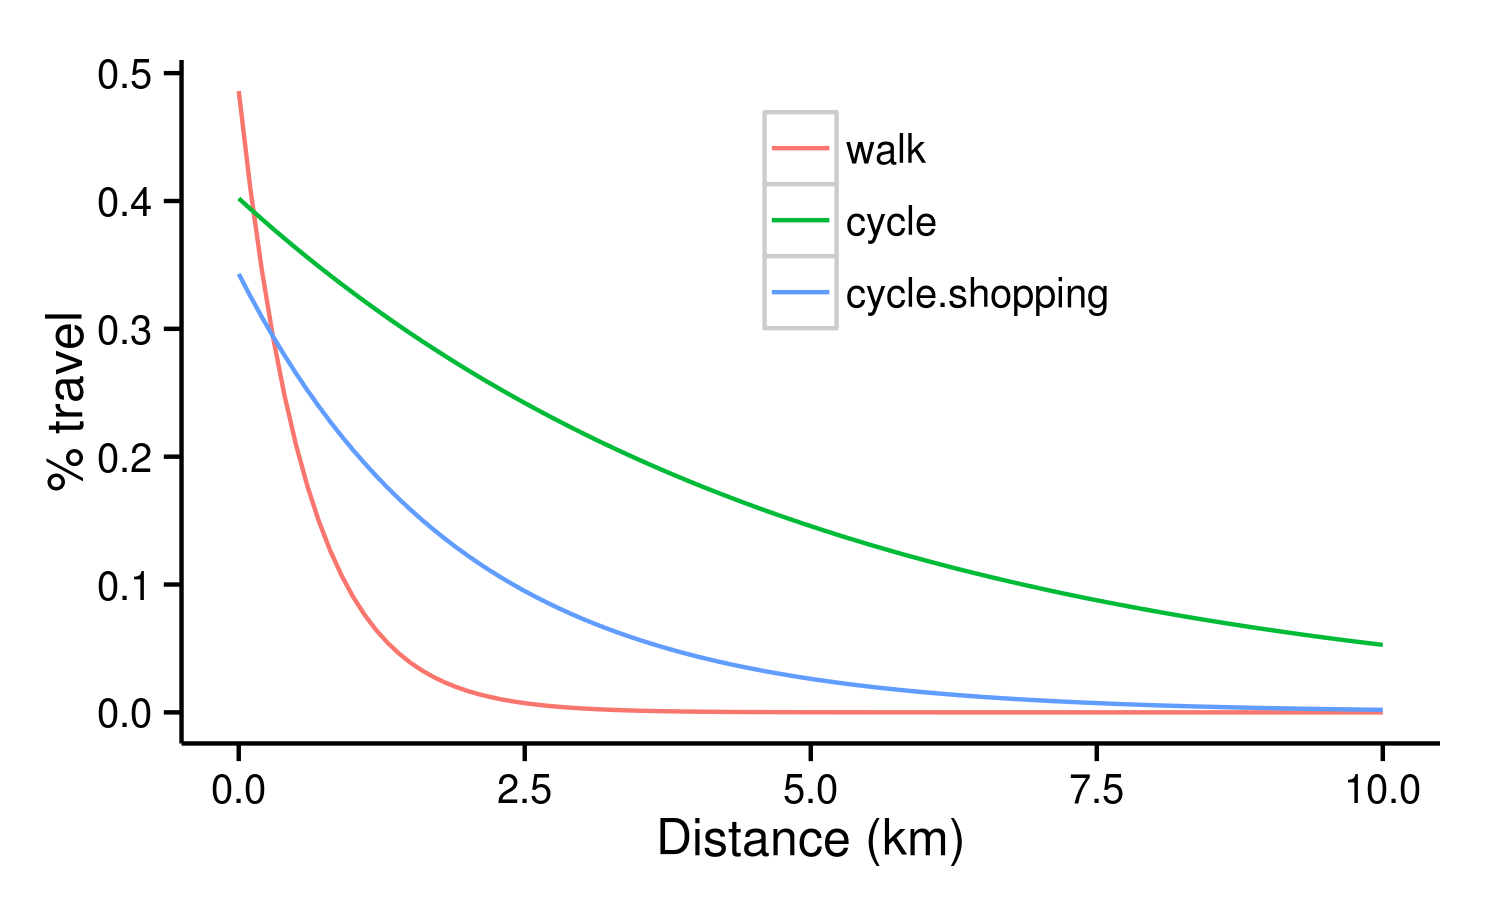
\includegraphics[width = 10 cm]{impedance}}
    \rule{35em}{0.5pt}
  \caption[Proportion of trips by active travel by distance and mode]
  {Proportion of trips made by active travel by distance and mode. Functional form
  from \cref{eimpedance}; parameter values taken from \citep{Iacono2010}.}
  \label{fimpedance}
\end{figure}

In summary, the sustainable mobility literature provides a strong foundation
for investigating energy costs in commuting. The emerging field of
active travel also has a strong interest in energy, although this is rarely
linked to the energy use of motorised modes. Sustainable mobility provides both
a world-view and methodological guidance for the thesis, yet is still only a
minor influence on commuting research overall, as shown in the subsequent section.

\section{Commuting research: individual to national levels} %%% only 1-2000 words
\label{s:commuting}
The energy costs of commuting depend on commuting behaviour.
As \citet[p.~297]{smith2011polycentricity}
put it regarding CO$_2$ emissions from travel to work, they are
``essentially a weighted combination of the mode-choice and travel distance
patterns.'' Understanding
the factors driving travel behaviour is key, therefore, to understanding
energy costs. `Behaviour' can be understood from a range of
perspectives, from the internal workings of the mind to the macro-economic
forces driving the type and spatial distribution of jobs
(\cref{fig:com-pyramid}). This section is structured to
reflect the multiple levels that affect commuter patterns.

Many important factors influencing the decision of whether, how and
how far to travel to work depend on the global economy, which is
largely beyond anyone's control \citep{Eisenstein2011}:
the price of crude oil, industrial
production\footnote{Production of
cars, trains and machinery, for example, is a prerequisite
for the construction and maintenance of transport infrastructure.
}
are all determined outside the sovereignty of any person or even
country, yet these factors, determined by the global economic system,
clearly have large knock-on effects on commuting patterns. National-scale
physical factors also play a role.
The transport network, shifting vehicle fleet efficiencies and the nation's
topography all help determine the ease with which
different commutes are undertaken, and their energy costs.
Large-scale political and
economic processes, such as congestion charges, fuel taxes
and house price gradients also affect commuting behaviour.
Zooming in on the local scale, the strength and nature of the local
economy will decide whether suitable jobs are available locally or
whether one's job search must go further afield.
Community and family ties could both make commuting distances shorter
(by providing support to family and friends searching for work --- the
``home-field advantage'' identified by \citealt[p.~100]{Simini2012}), or longer
(by creating a disincentive for people to move closer to where they
work \citealp{Green-1999-ld-commute}).
At the simplest level, however, the decision to get up in the morning
and commute to work is ultimately made by individuals \cref{fig:com-pyramid}).

\begin{figure}[htbp]
  \centerline{
    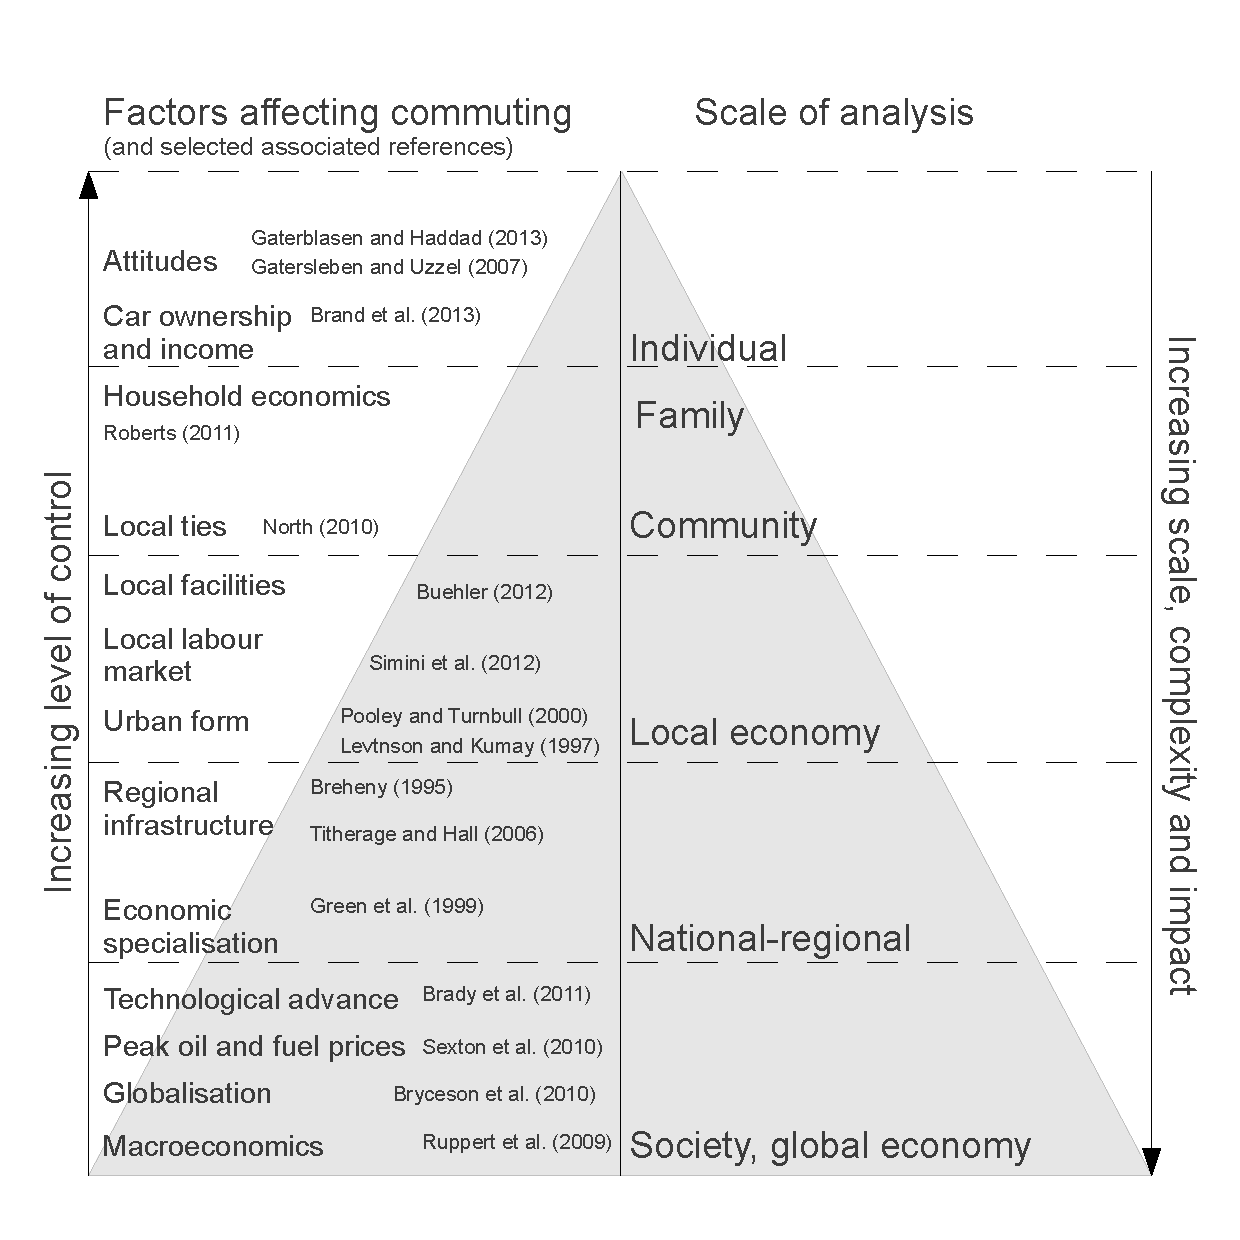
\includegraphics[width = 10 cm]{commuting-research-image2}}
  \caption{Schematic
for organising research commuting research by scale.} %%% could update with methods
  \label{fig:com-pyramid}
\end{figure}

\subsection{Personal factors: psychology, family and community}
As Chris Fisher's story demonstrated (\cref{s:realities}), human beings are not
merely economic machines motivated solely by money. We make decisions based on
a wide and interrelated range of factors \citep{Pinker1997}. Some are instinctive, others
are carefully planned \citep{Kahneman2012}. 
%Within this array of factors
%money tends to play an important role, as do family considerations
%and proximity to friends and one's home town.
While money plays an important role, it is within an array of 
factors along with family considerations and proximity to friends and home.

In some ways, long-distance commuting is the ultimate
manifestation of the conflict between
work and family life. If money were the only objective, people would be far more
mobile, willing to pack their bags and leave to live near better salaried jobs
whenever opportunities arrive. This is obviously not the case:
``job relocation almost always involves a move not only of one
individual's job, but also of his/her household's home and of jobs/schools for other
household members''
\citep[p.~52]{Green-1999-ld-commute}.\footnote{This
decision, to move for personal reasons rather than work,
is also well-expressed in everyday speech:
``I'd much rather
have a crap job and be with Richard than have a good job and be miserable'', as one
person told me (Emma, 2013, personal communication).
}
Over the past 50 years, perhaps due to the perceived social costs
of this upheaval, job relocation has increasingly
\emph{not} led to house relocation, but longer commutes instead
\citep{Green-1999-ld-commute, Nielsen2008}.

This trend has been labelled the `commuting paradox' due to the
seeming irrationality of the decision 
to spend much of one's time travelling to work and back \citep{Stutzer2008},
in face of evidence of negative impacts on well-being \citep{novaco1990objective}.
Approaching the problem at the individual level makes sense:
people are not economic machines,
yet assuming that people make a personal cost-benefit analysis for each
available option allows the powerful tools of microeconomics to be used. Applied to
commuting, each individual would evaluate all work-home (and
hence commuting) options and select the
best \citep{Stutzer2008}.\footnote{Mysteriously,
as the authors of the `commuting paradox' point out, this cost-benefit analysis is often
performed in a less that rational way, leading to commuting costs
(predominantly on unquantified well-being) that far outweigh the benefits
in many cases \citep{Stutzer2008}.
}

Research into commuting at the individual level generally uses psychology
(e.g.~\citealp{van1998social}) or microeconomic theory (e.g.~\citealp{van1999job}) to explain
\emph{why} people choose their commuting behaviours.
Yet the level of analysis is generally weaker when it comes to describing
\emph{how} commuting patterns --- the aggregate pattern of many individual flows ---
are configured and how much energy or other resources these patterns
use relative to other activities.
The relationship between commuting and larger scale processes
is generally not considered in individual-level studies, although
there is a move towards more holistic understanding of individuals.
One study that analysed both environmental and psychological
determinants of individual level commuting behaviour found conclusive evidence
(from a sample of 130 university students) that ``cognitive variables play
a more important role in the prediction of active commuting than do environmental
variables'' \citep[p.~9]{Lemieux2009}. Because of the non-geographical nature
of this study and its small sample size, however, it provides little evidence
on the factors related to \emph{aggregate-level} variability in commuter flow
patterns. Local, regional and national-level studies are needed.

% The psychological literature on commuting sheds some light on
% this commuting paradox.
% \citep{Brand2013}
% \citep{Gatersleben2010}
% \citep{Roberts2011}
\subsection{Behavioural economics and its impacts on commuting}
Behavioural economics seeks to explain a large part of human behaviour in advanced
capitalist societies where making money is often (implicitly or otherwise) seen
as the number one \emph{raison d'etre} of life \citep{Eisenstein2011}.
The underlying assumption that human beings are rational beings
has of course come under attack from many quarters. To take one 
example, ``There is probably no other hypothesis about human behaviour [than
economic rationality] so thoroughly discredited on empirical grounds that still
operates as a standard working assumption in any discipline''
(Anderson, 2000; cited in \citealp[p.~34]{Exel2011-b-ec}). 
Despite these criticisms it is easier to create testable models in economics 
than the social sciences (Perman, 2003).
%Despite
%these
%criticisms, and the fact that the idea of an `economic man' is abhorrent to many
%people's better instincts, a clear advantage of economics over other social
%sciences is the possibility to formulate and test quantitative relationships,
%to evaluate the extent of the models' deviance from reality \citep{Perman2003}.

Indeed, many economists would be quick to point out that the term `economics'
has been conflated with what is in fact `neoclassical economics' in the public
consciousness and in other academic disciplines.
It has been argued that it is only with the recent
focus on money exclusively (instead of the physical reality that underpins
its value) that utility and profit have been conflated \citep{porritt2007capitalism,
Eisenstein2011}.
Clearly, it is not money per se that affects commuting energy costs, but
its indirect influence on behaviour, which is rarely direct. It is for this
reason that behavioural economics is the
branch of the discipline with most insight into travel to work patterns.
At its most tempered, modern behavioural economics completely accepts that much
of human behaviour follows a rationality other than the profit
motive. Many behavioural economists acknowledge the findings of Nobel
Laureate Daniel Kahneman, neatly summarised in the
book \emph{Thinking, Fast and Slow} \citep{Kahneman2012}, which
explains that humans are servants to both cool rational thought processes
(when `system 2' is dominant) and also to quick-fire decisions based on
spontaneous urges and heuristic reasoning (when `system 1' is dominant). The
caveat in the quantitative analysis underlying economic analyses
becomes ``when humans are acting
rationally, with the objective of maximising profit'' which is only some of the
time.
% (the rest of the time providing a convenient explanation for model errors).

If these limitations are understood, behavioural economics can provide a powerful
framework for explanation. The
framework is consistent with anecdotal evidence about the reasons behind travel
behaviours (e.g.~Chris Fisher's decision not to move to Hereford because
commuting to the Tyrrel's crisp factory would then become too expensive) and
the observed behaviour that people react predictably to price signals.
The framework can also be called upon to explain more general (and less
testable) trends, such as the increasing dominance of the car throughout the
20$^{th}$ century: ``One important reason for the automobile's increasing
dominance in passenger transport is that ... the price of car travel relative
to public transport has largely remained steady while the (system) quality of
car travel has considerably increased relative to public transport''
\citep[p.~149]{Exel2011-b-ec}. % p.149 in the book in case it's different
Far from assuming humans are soulless economic machines,
such explanations, taken as descriptors of aggregate behaviour,
% (not that of specific individuals),
assume citizens are simply careful with their cash.
Such explanations are supported by multiple studies of transport elasticity
(e.g.~\citealp{goodwin2004elasticities}).

\subsection{The local and regional economy}
The idea that localised environmental factors can
influence behaviour patterns has a strong tradition
in geography.
In terms of the impact of local factors on commuting, existing
research has focussed on transport infrastructure, the built
environment,\footnote{The
built environment is defined as ``equipment, facilities or infrastructures in
one's environment'' that influence travel behaviour by \citet[p.~2]{Lemieux2009}.
The built environment can thus be seen as a superset of transport infrastructure,
which includes features such as parks, street lights and even showers designed
to encourage running or cycling to work.
}
topography and local economies, as well as the more abstract concept of
`urban form'.

A common research strategy for exploring these links is to take aggregate travel
behaviour in different areas as the dependent variable and set-up a
multiple regression model to identify which factors can best explain its variation.
This strategy has provided a number of insights into commuting
behaviour and its dependence on geographical factors:
\begin{itemize}
 \item \citet{Buehler2012} ran a logistic regression model and found that
 the provision of showers and bicycle parking by employers (which
 had not previously been included in regression models of commuter behaviour)
 were significantly related to the chances of respondents cycling to work.
 The provision of bicycle lanes and free car parking also had large
 impacts on the odds ratio of a person cycling in the expected
 direction, supporting past literature on the matter. Significantly, this
 study also combined household-level variables; it was found that a high number
 of bicycles (and low number of cars) per household member also increased the
 propensity to cycle, as did high income and `white' ethnicity.
 \item  \citet{Titheridge2006} used distance of commute as the dependent variable
 in their study of commuter patterns in the East of England. It was found that
 distance from London, social class and level of car ownership in each ward
 affected distance in the expected ways. Population density, which would
 be expected to be associated with lower energy costs based on the `compact
 city' concept, was positively associated with commuting distance in their model.
 This contrasts the idea that bunched-up living is a panacea for travel costs and
 was explained by \citet{Titheridge2006} in terms of accessibility to transport
 infrastructure.
 \item \citet{Muniz2005} performed a regression analysis exploring the impacts of urban form on
 the `ecological footprint' (which is closely related to energy use) of commuting
 in Barcelona Metropolitan Region. It was found that, for the 163 municipalities
 that constituted the case-study area, low population densities, high `accessibility'
 (which seems to have been defined simply as distance from central Barcelona)
 and high average income all were positively associated with the dependent variable.
 Although this study was conducted at only one scale (it may suffer from the
 ecological fallacy and does not prove causality), the authors concluded that
 factors relating to urban form ``have a greater capacity to explain municipal
 ecological footprints variability than other factors'' \citep[p.~511]{Muniz2005}.
\end{itemize}

Such studies, which use geographical zones as the unit of analysis,
have revealed some of the factors that are closely related to certain commuting
patterns. Some of these, such as propensity to cycle and distance to workplace,
have important energy implications. When the independent variables include
factors over which policy makers have some degree of influence, such as
employers' provision of showers investigated by \citet{Buehler2012}, the
findings can be used to predict changes resulting from new policies. Even in
cases where the independent variables are largely beyond anyone's control ---
such as population density and home-work distances ---
regression analysis can be useful: it can be used to identify anomalies
where commuting patterns differ greatly from what would be expected based on
explanatory variables alone. In these cases, it must be acknowledged that
other processes are in operation, which can lead to new avenues for research.
However, regression analysis used in this way is limited:
causality is not proved; relationships may not hold at different levels of
analysis; and standard regression does not take space into account
(spatially weighted regression can be used to tackle this problem).
Partly to overcome these limitations, a number of other strategies have
been used to explore the geographical determinants of commuting behaviour.

In a study of commuting behaviour in northern Sweden, descriptive statistics
and maps were used to characterise commuter patterns in the region \citep{Sandow2008}.
Making use of the abundant
anonymous spatial microdata made available by the Swedish state, an
individual-level logit model, with long or short distance commute
set as the binary variable,
was used to explore the reasons for and impacts of the observed patterns.
It was found that people living in more sparsely populated areas
were more likely to travel far to work living in dense areas.
This was as expected (but in contrast to \citet{Titheridge2006}).
The individual-level data allowed for the investigation of socio-demographic
variables: education and income were associated with longer commutes.
Interestingly (in contrast to UK data), commuting distance decreases
with every age group above the 16-25 band. Gender differences were also
apparent: men travelled further than women and the impact of marriage and
children on the probability of commuting far was greater on females. Thus
it was concluded that family
commitments ``constrain women to a higher extent than men''
\citep[p.~24]{Sandow2008}.

% Urban form: \citep{Pooley2000commuting}
% \citep{Levtnson1997}
% \citep{North2010585}
% The importance of infrastructure has been noted in a number of studies.
% \citep{Titheridge2006} 

\subsection{National and global considerations}
While regional approaches have tended to focus on detailed sub-regional factors
affecting commuting, national approaches tend to be broader. The large
quantity of data available (albeit often at a high level of spatial
aggregation and low temporal resolution) make the national level
well suited to analysing shifts over time and persistent patterns within commuter
flows. Larger study areas also shift attention towards universal concepts,
that should, in theory, apply anywhere with similar underlying conditions.

In the context of the compact city debate, an individual-level regression
model involving 47,000 people across the US was undertaken by
\citet{Levtnson1997} to ascertain the impact of population density on
travel to work distance and time (and hence average speed also). A wide range
individual and geographical
factors (the latter aggregated at the level of Metropolitan Statistical
Areas (MSA), roughly equivalent to country level in the UK) were
used as explanatory variables. These were
carefully selected based on theory and previous findings. They
included a measure of polycentricity (the number of `activity centres' --- meaning
employment centres --- in each MSA), population growth rate and three variables
to quantify the transport technology in use in each area. It was found that for
car drivers, travel speed and distance were negatively associated with density. Time,
which had received little attention in the compact city debate previously, was found to be
negatively associated  increased residential density up to a certain limit
and then actually increase above this threshold. It was concluded that
this indicates diminishing returns as the density of settlements increased 
if cars are the main form of transport, due to congestion. Public
transport users, by contrast, ``displayed a negative relationship between travel
time and density both above and below the 10,000 ppsm density threshold'',
suggesting that these modes are less affected by traffic (and hence more attractive)
in dense urban areas \citep[p.~168]{Levtnson1997}.

Building on these findings, \citep{Levinson2012}
returned to the question of the factors affecting commute time in US
MSAs with updated datasets and more sophisticated tools for analysis.
It was found that accessibility was the major determining factor of
travel to work characteristics at the MSA level, and had a strong negative
association with average time and mode share of cars. Accessibility
(a slightly refined version of which was used in the final model) was defined,
for given time thresholds, as follows:
\begin{equation}
 a_t = \pi \times \left[ \frac{V_n \times t}{Q} \right]^2 \times p_{emp}
\end{equation}
where $V_n$ is average network velocity, $Q$ is circuity ---
see page xix for definition and \cref{fig:routes} for illustration ---
and $p_{emp}$ is the urban density (measured in jobs per km$^2$). A number of other
mathematical entities were used to define the transport network, the most
influential of which were treeness (roughly speaking, the proportion of the network going to
new places), connectivity (measured in five metrics, from alpha to gamma) and
circuity. The relevance of \citep{Levinson2012} for this thesis is that it
provides strong evidence to suggest key aspects of the journey to work are
influenced by road and settlement factors, and a set of tools for measuring
and assessing the effects of these factors. These techniques are not
used in a model of commuter energy use in the case studies presented in
this thesis, but could be in the future.

% Also at the national scale, \citet{Turnbull2000} used retrospective
% questionnaires to assess the changing nature of travel to work over time.
% The sample size was small 

Commuting has been studied and understood from a wide range of
perspectives. For the purposes of this thesis, insights are taken from economics,
ecology, and transport geography. The first assumes commuters to
be free thinking utility maximisers \citep{Sexton2011}; the second sees humans
as ``mobile, interacting animals'' who ``are no different from our fellow
species'' \citep[p. 40]{Brockmann2012}. Transport geography tends to be
agnostic in its explanatory framework, taking insights from the spatial
structure of transport networks, supply and demand centres, and the physical
environment \citep{Rodrigue2009}.
Interestingly, considering the ubiquity of commuting worldwide, no
research into commuting as a global phenomenon could be found, let alone
systematic comparisons between nations.
This suggests that there is a research gap in the area of international
commuting studies, which may be partially filled by a comparison of the
UK and the Netherlands later in this thesis \cref{sinternational}, as
recommended in the conclusions (see \cref{sfurther}).

\section{Energy use and CO$_2$ in transport studies}
\label{s:energy}
The traditional reasons for interest in commuting and  personal transport
more generally include its links to urban structure, industrial location,
productivity of workers and  quality of life. Economic factors have
tended to be dominant in past research,
but energy use and its environmentally destructive impacts,
predominantly quantified in the form of greenhouse gas emissions,
% \footnote{The term
% `evil twin' is used here because emissions almost always result from
% energy use in transport, yet only the latter is seen as a `bad' thing.
% Energy use can be seen as a good thing when used as a measure of economic
% activity.}
are increasingly becoming a focus for transport researchers \citep{Chapman2007}.
Although CO$_2$ production is a direct result of energy consumption,
depending on emission factors (\citealp{Defra2011}; see \cref{fgco2}), some studies continue to
treat them as separate issues. \citet{Boussauw2009}, for example,
calculate the energy costs of commuting in Flanders, but nowhere does
the paper mention the link to climate change: results are also, in essence,
a map of CO$_2$ emissions due to commuting, relevant to EU targets.
On the other hand,
it is possible and equally valid (if one's primary concern is climate change)
to only quantify CO$_2$ emissions and acknowledge
that the results essentially show energy use \citep{smith2011polycentricity}.

\citet{Simonsen2011} harnesses the knowledge that energy use
and greenhouse gas emissions are two sides of the same coin to use the
same energy analysis model to quantify both. In their analysis of cars in Norway,
it was found that only electric vehicles powered by renewable
sources (hydro-electric plants in this case, which are bountiful in Norway)
performed well. The approach taken in this thesis follows
\citet{Simonsen2011} in seeing the link
between energy and emissions.
% but takes it even further: the former is seen
Moreover, it is assumed that the former is a a close enough proxy of the latter
at the system level that only energy use needs to be
calculated to gain an understanding of
both.\footnote{`At
the system level'
in this context means emissions arising from knock-on impacts of
interventions in the transport system are taken into account.
For example, if rapid uptake of electric cars leads to slower phasing
out of fossil fuel fired power plants, this would constitute
additional emissions at the system level that are not included in
official emissions inventories.
}
This prevents the complexity of having to report two (very highly correlated)
sets of indicators for the energy and emissions impacts. They are assumed to
be essentially the same thing.

Underlying drivers of this interest in energy use in transport and
associated emissions include peak oil and climate
change (\cref{Chapter1}). This attention has led to 
methods and findings directly related to the thesis.
% The work described in the following section is therefore of practical use.
% Describing the methods of, and questions raised by, this body of literature are
% therefore priorities of the subsequent section.
Although there has been a recent proliferation of interest in the contribution of
transport energy use to climate change \citep{Schwanen2011}, the topic
has  received attention, intermittently, over many years. Interest seems to
have peaked during the 1970s,
following the major oil crises of that decade \citep{Greer2009}. Since then the
topic has largely been confined to the following fields:
\begin{itemize}
 \item Urban sprawl:
 the phenomenon of low density housing, also known as suburbia, is highly car
dependent and has attracted attention investigating its impacts on transport energy
use. The antithesis to this is the `compact city'. Investigation of continuum between
these two extremes has led to many insights on the impact of urban form on transport energy use.
\item The energy costs of transport modes: quantifying which modes of transport
use most, and least energy per unit distance, typically per passenger, vehicle or
tonne kilometre: $pkm$, $vkm$ or $Tkm$.
% \item The `compact city' debate, in which the hypothesis that high density
% settlements are more energy efficient, due largely to transport.
% \item Life cycle analysis (LCA) and studies of the relative importance of
% embodied energy in transport systems.
\item The climate impacts of transport, usually quantified through estimates
of the quantity of CO$_2$ directly emitted by vehicles.
% \item The field of `energy and equity', which investigates the impact of
% unequal access to powerful machines for personal travel and social inequalities.
\end{itemize}
Transport and energy use is a broad area of research, so it
is inevitable that not all of it fits neatly into these four categories. A fifth
category, miscellaneous studies on transport an energy, will emphasise this
diversity of approaches, and touch on the interdisciplinary nature of the work.

\subsection{The energy costs of urban form: urban sprawl and compact cities}
The links between urban form and consumption of fossil fuels (primary energy)
have been of interest since at least the 1940s, especially amongst utopian town
planners \citep{Steadman1977}. Of the various types of urban form under
consideration, from the fictional `City of Efficient Consumption'
\citep{Goodman1947} to the `compact city' \citep{Breheny1995}, none have
received more critical attention than that of urban sprawl \citep{Marshall2008}.
Urban sprawl has long been identified as an energy intensive settlement
pattern, with social and environmental knock-on effects: ``Urban sprawl not only
consumes more natural ecosystems and has a higher cost per unit of development
in both money and materials, but once completed it requires higher inputs of
energy and generates more air and water pollution'' \citep{Bormann1976}.

Such statements may seem obvious, yet without evidence questions about
the extent of the
problem, and how to mitigate it, remain unanswered. This is a key motivation
behind methods which seek to measure aggregate energy use over space, and
provide breakdowns of how much energy is used where, and insights into why.
% (Example of overall energy use)
One implicit assumption underlying much of this research is that
energy use is \emph{the} defining
variable of a settlement and hence requires most attention.
This reasoning was stated explicitly by
\citet{Marique2012}, who note that despite the primacy of the transport sector
in driving up energy use in sprawling suburbs, ``transport energy consumption
is rarely taken into account'' (p.~1). In response to this negligence, the authors
quantify the average transport energy costs in four settlements, based on travel
statistics. Their analysis shows commuting to be the most
important determinant of transport energy consumption in Belgium. Commuting
consumes more than double the amount of energy (4000 to 6000 kWh/p/yr) 
than the next largest transport energy user (trips to school)
\citep{Marique2012}. These findings lend support to the topic of this thesis and
encourage further analysis of energy use in personal travel overall.

Despite the use of census data, \citet{Marique2012} present their findings only
at high levels of aggregation, for entire settlements. The \emph{distribution}
of energy consumption within the areas is not considered. Nor are the
\emph{types} of people responsible for high energy use for commuting. These
gaps in their research suggest more detail would be welcome: providing a method
to calculate the energy costs of commuting at lower geographies that is capable
of providing breakdowns of energy use at the individual level would constitute
a step forward for this research.

\subsection{The energy costs of different transport modes}
The relative energy use of different ways of travelling per unit distance
or time has been of interest
to researchers at least since the 1800's when \citet{tredgold1835practical}
was taking measurements from railway engines to ascertain their coal
consumption. A more universal approach to energy use in transportation
was taken by \citet{Gabrielli1950}, who characterised the energy performance of
different modes, for given speeds and loads. This model included jet fighters,
helicopters and even a horse, as well as more traditional vehicles such as
cars, bicycles and trains. Although largely unnoticed by the academic
community (it has been cited 11 times according to Google Scholar), this
paper was seminal in its approach to comparing widely varying forms of
transport, and the findings still largely hold today (although efficiency
gains have been made) \citep{yong2005price}. An updated analysis, which uses
a simpler energy performance metric, kilogram-metres per Joule, multiplied
by speed ($kg*m^2/J/s$) applied the method
to a wide range of modern vehicles, confirming the relatively poor energy
performance of cars in comparison with trains and bicycles (\citealp{Radtke2008},
\cref{fgabrielli}). This is a recurring them in \cref{Chapter5}.

\begin{figure}[htbp]
  \centerline{
    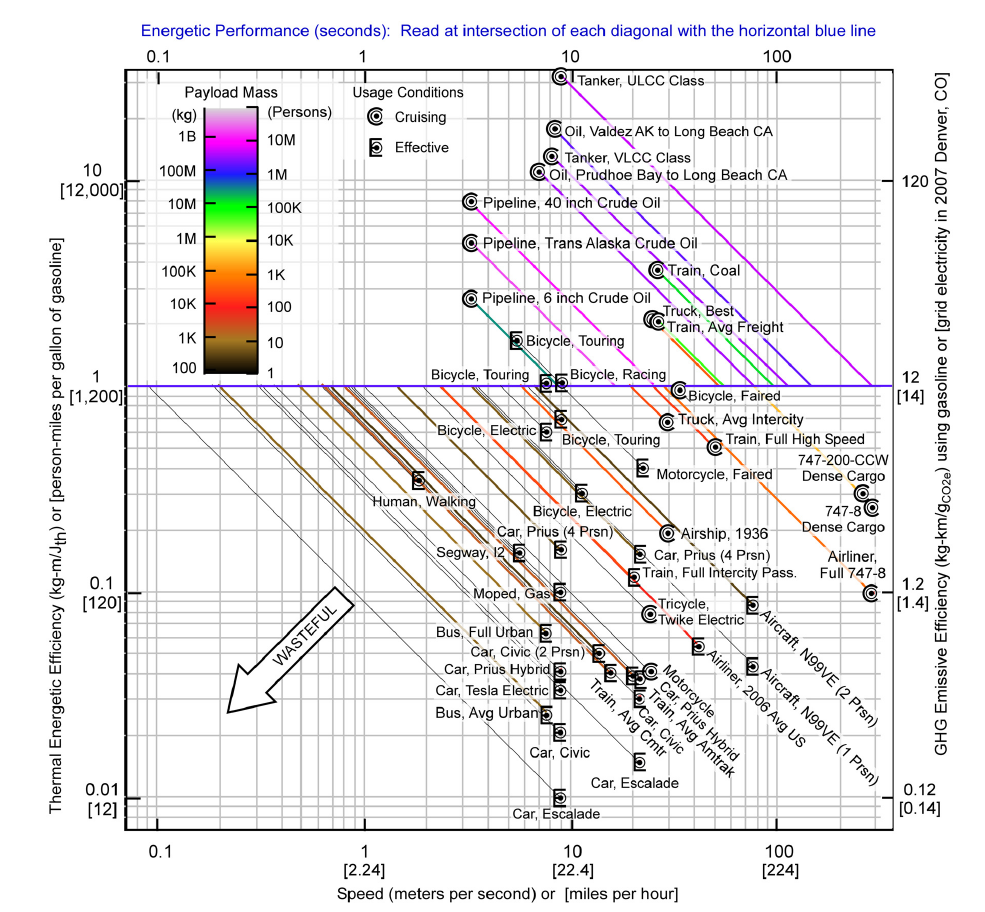
\includegraphics[width = 13 cm]{gabrielli}}
  \caption{Energy performance of different modes, from \citep{Radtke2008}.} %%% could update with methods
  \label{fgabrielli}
\end{figure}

\citet{Gabrielli1950} and its successors made large advances in understandings
of the relative energy costs of widely different transport modes.
It is therefore surprising that methods and findings stemming from this
work are not more frequently used in transport studies.
One limitation of the research area is that it omits indirect energy impacts from
the analysis.
This is problematic because vehicle and infrastructure manufacture obviously
require large amounts of energy: inclusion of direct energy costs only
``might lead to serious faults in estimating environmental impacts of new
infrastructure or modal shift policies'' \citep[p.~23]{Wee2005}.
A pioneering paper that sought to overcome this issue quantified
both the direct and indirect
energy costs per unit kilometre of the main US modes of personal travel shortly
after the 1973 oil shock \citep{Fels1975}.

In hindsight, Fels' research seems to have stood at the beginning of a
research area, dedicated to assessing the wide-boundary energy impacts of
personal travel. Key papers in this area include \citet{Lenzen1999}, who used
updated versions of Fels' early methodology to calculate the total energy and
emissions impacts of the Australian transport system and  \citet{Ramanathan2000}
used a new method (`data envelope analysis') to investigate
the relative energy costs of Indian road and rail transport.
% The analysis was
% novel in that it took into account both freight and passenger transit in
% the analysis, leading to the finding that rail efficiencies have continuously
% improved, while road transport efficiency has plateaued since the late 1980s.
Another group of researchers have researched essentially the same
issue, but with different methodologies and terminologies
(the `well-to-wheels' approach) from the
life cycle analysis (LCA) perspective (e.g.~\citealp{wang2002fuel};
see \cref{sfuelem}).
Because research rooted in LCA tends to be
concerned with emissions rather than energy use per se, it is
of slightly less relevance to this thesis.
Surprisingly, there seems to be
limited overlap between the well-to-wheels approach and the aforementioned
system-level energy use studies.
Despite the activity of these research areas, 
there has been limited uptake of system-level energy
cost estimates in transport studies overall. Direct emissions and
their climate impacts have received more attention.

\subsection{The climate impacts of transport}
Since 1985, when Professor James Hansen of NASA's Goddard centre testified
to the US congress about the threat posed by climate change, there has
been a growing concern about the issue from all quarters, including the media
\citep{Boykoff2007}. While media insistence on `balance' seems to have actually
led to bias in climate change reporting, providing excessive coverage to contrarian
views \citep{boykoff2004balance}, academia has largely risen to
the challenge in practical terms. A multitude of articles has been written on how to
reduce emissions in everything ranging from catering \citep{gossling2011food}
to the Indian cement industry \citep{kumar2010environmental}.
Acknowledging that transport is responsible for roughly a quarter of emissions,
researchers in the sector have been no exception.
Modelling scenarios of future change proposing new policies
for emissions reductions are now common themes in the transport literature
(see reviews by \citealp{Chapman2007} \citealp{ross2010analysis}).

Without delving further into this large and diverse body of literature,
a few generalised criticisms of it can serve to
highlight where improvements can be made. It is acknowledged that
these observations do not apply to all research into
transport and climate change. The reason for voicing these concerns,
summarised in the bullet points below, is that they
help focus attention on areas within the field lacking in
coverage.
% Their consideration has contributed to the energy approach
% to commuting presented in this thesis in the following ways:
\begin{itemize}
 \item Transport and emissions studies have tended to focus exclusively on
 direct emissions, to the detriment of understanding of the system-level or
 `embedded' emissions resulting from transport policies,
 such as road construction and vehicle
 manufacture \citep{Lenzen1999, Wee2005}.
 \item Because of the focus on the national-level, papers in the area
 could be argued as offering little in the way of support to local and regional transport
 planners. This is an important oversight because local and regional-level
 transport planners vastly outnumber national policy makers (in staff, if not
 in terms of political influence).
 \item The various scenarios of the future often appear to be overly academic,
 arbitrary and unrealistic. This is
 problematic because impenetrable models and scenarios
 may prevent engagement and interaction with the
 possible futures presented, by either the public at large or policy makers.
 To overcome this issue, participatory models
 such as that published online by the Department of Energy and Climate Change
 (\href{http://2050-calculator-tool.decc.gov.uk/pathways/11111111111111111111111111111111111111111111111111111/primary_energy_chart}
 {\color{blue} 2050-calculator-tool.decc.gov.uk}) have been advocated
 \citep{fulton2012exploring}.
\end{itemize}

Despite these issues, this thesis fits within the field: although the emissions
benefits are not calculated explicitly, it is not a large jump from energy
costs to emissions (CO$_{2eq}$ output
would be easy to estimate, based on the
emissions factors present in \cref{Chapter5}). The efforts to estimate
system-level energy costs of different modes presented in the same chapter
are aimed at overcoming the focus on direct emissions alone, prevalent in the
transport-climate change literature. Regarding scale, in some ways it makes
sense that many of the studies in the area operate at a large scale
because climate change is inherently a global issue.
The problem is that there is an excess of studies that operate only at the
national level, with relatively little work focussing on larger or smaller geographical
unit of analysis. The methods
presented in this thesis are well-suited to smaller geographical unit areas, although
they can also be applied to nations (\cref{Chapter6}).
The methods presented in this thesis are not participatory (unless one is
willing to learn to code in R and apply it to spatial microsimulation!).
However, effort has been made to make the code and data underlying the
models as accessible as possible.\footnote{See
\url{http://rpubs.com/robinlovelace}, which contains links to
reproducible result, via sample code and data. Github has also
been used to make some experimental analyses available.
}

% \subsection{Assessing the energy impacts of political intervention} \label{spintervention}
% !!!

\section{The energy impacts of commuting} \label{sdisciplines}
The intersection between these two study areas, each large in its own
right and with substantial interaction, is surprisingly small.
As described in the previous two sections, major advances in understanding
commuting behaviour and energy use in transport have been made.
The problem is that these insights into commuting are often not
translated into energy use
estimates.\footnote{This step is in fact
relatively straightforward, once the energy use of different modes is well-known
(\cref{Chapter5}).
}
Or, conversely, existing estimates of energy use of different modes and
other personal variables are not combined with readily available
commuting statistics. The energy costs of commuting is not a
`pure' research area, in the sense that it relies on combining data from
sources that often are not linked.

The study that most closely fits the title of this section
was based on aggregated census data from Flanders. Without relying on
regression analysis  or sophisticated statistics \citet{Boussauw2009}
provided a detailed account of the factors linked to areas with
high and low average commuter energy costs. By mapping average
energy consumption per person per day (ranging from almost zero
to above 30 kWh/p/d) for small administrative zones, the impacts of
modal split (minimal), distance (``paramount'') and urban morphology and
infrastructure on energy use for commuting was determined. These are new
and important findings that need to be tested in other countries
and at different scales
before they are accepted as `universal' relationships that can form the basis of
policies worldwide. It was concluded that
``the energy performance of the transport system is an important approximate
indicator for the sustainability of a spatial structure'' \citep[590]{Boussauw2009}.
This observation was a major motivation for the subject matter of this thesis.
%!!! requote this elsewhere???
The political implications of the research are wide-ranging: the prevailing
focus on mode-split in Belgium (and in many other countries, including the
UK where uptake of cycling has become a major political issue) seems to be misguided.
Governments should instead focus on enabling their citizens to live closer to their
place of work.

\citet{Boussauw2009} did not provide `further research' type conclusions. However,
the arguments made throughout for a greater role for energy-based metrics of
transport system performance and sustainability clearly imply that more
research measuring energy use in commuting is needed. The paper therefore
provides a strong intellectual foundation on which this thesis is built.
The methodological guidance was limited as the analysis was quite simple.
From this was taken the importance of seeing method as a means to an end,
rather than an end in itself, an issue that has been debated in academia for
many years. 
%% surely there's another study that fits here???!!! looking good though.

% \subsection{Energy use and transport poverty} 
% One of the earliest investigations into the
% links between energy intensive modes and social and economic disadvantage
% was Ivan Illich's book \emph{Energy and Equity}
% \citep{Illich1974}. Since then, the causes identified by Illich for growing
% inequalities in personal mobilities and `power' --- the ever increasing speed
% with which the economic elite can travel, powered by fast cars --- has grown
% and plateaued. % would like to re-add this, at some point!!!
% 
% \citep{Sustrans2012}. %

% Commuting is an inherently spatial activity, as its purpose is % valuable!!!
% to transport people from A, their home to B, work.
% This, combined with readily available official data sources
% on commuter flows, make the phenomenon well suited for study
% within the field of transport geography. This field aims
% to explain ``the socioeconomic, industrial
% and settlement frameworks within which transport
% networks develop and transport systems operate''
% \citep{Hoyle1992modern}. %%% Citation added.
% The focus on explanation rather than mere description
% makes the field a rich source of ideas about \emph{why} transport systems,
% and more specifically commuter patterns, are the way the are.
% Plough on with examples from the literature

% Commute minimisation \citep{Buliung2002}
% 
% The concept of `activity space' is another key concept
% used by transport geographers... \citep{Buliung2006}.

% Transport geography is inherently multidisciplinary,
% and has contributed to wider debates started in other fields.

% \citep{Marique2013}
% 
% Despite the theoretical bias in Transport Geography noted at the beginning of
% this section, there have been substantial methodological contributions to the
% analysis of commuter patterns. The methods to evaluate different
% types of estimate of route distance (GPS, shortest route algorithms via
% GIS and straight-line distance) presented by \citep{Stigell2011}.
% Their result that self-report distance is the least reliable provides
% useful background for assessing the reliability of the input data
% used in this PhD. (Census data are straight-line distances by
% postcode, the survey data is self-reported route-distance.)

% \subsection{Non-academic contributions to commuting research}
% The above research is based predominantly in the realm of academia, written by
% University scholars and published in academic journals. The advantages of this
% `academic model' of research are clear, and have been implemented throughout
% this thesis. These include:
% \begin{itemize}
%  \item Traceability of sources of information --- hence the inevitable in-text
% references and lengthy reference lists that accompany academic research.
% \item Reproducibility of results --- academic writers must clearly state what
% they have done, why and report the results in a way that could be replicated,
% given the correct conditions.
% \item Impartial writing style --- academic writing is different from more
% creative styles, in that ideas must be ordered logically and artistic elements
% minimised in favour of clarity \citep{oshima1997introduction}.
% \end{itemize}
% 
% Because commuting is such an important part of the daily routine for millions
% of people, it has received much attention from outside academia too.
% Literacy has improved worldwide and
% opportunities to publish (most recently with the emergence of paperless
% E-books) have multiplied, so it is impossible to hope to have encountered even
% a tiny fraction of the totality of material written about
% commuting.\footnote{This
% could be interpreted as an additional advantage of the academic publishing
% model: it is relatively cohesive self referential compared with the tangled
% mass of non-academic writing. The latter is not ordered into neat searchable
% databases that is connected by a formal reference system in the same way that
% academic papers are.}
% What follows therefore is a concise summary of `lay' works on
% commuting that have been discovered, usually by coincidence, and that
% contribute information or understanding to the topic energy costs of commuting.
% 
% \citet{Orloff2002-60-second-commute} provide a self-help guide on telecommuting
% for those wishing save time and money.

While \citet{Boussauw2009} were writing from the perspective of transport
geography, the primary concern being spatial variation of energy costs,
the issue of energy costs has also been tackled from the perspective of
mainstream economics. \citet{Sexton2011} paper set out to
test a hypothesis: that the 2008 sub-prime mortgage crisis was triggered
by high liquid fuel prices. The mechanism for this was commuting energy costs ---
those who live closer to their place of work were found to be less affected.
This was shown through a number of maps illustrating the change in average
house prices over space. Areas furthest from employment centres had the greatest
falls, whereas house prices in more central locations were relatively unaffected.
This study demonstrates the importance of energy costs of commuting,
not just in abstract terms of environmental impact or global resource depletion,
but in terms of direct impacts on peoples' lives. No attempt is made to
replicate the economic methods used by \citet{Sexton2011} in this thesis.
However, \cref{svul} was heavily influenced by the paper. It takes from
\citet{Sexton2011} the need to asses potential future impacts of high oil prices
on different social groups.

\section{Commuting and energy use research: tools of the trade}
\label{s:tools}
The previous section illustrates that energy use in commuting can be seen in 
at least two different ways: a dependent variable influenced by geography, or
an explanatory variable affecting household expenditure.
Many other ways of looking at commuter energy use are possible and each
would suit different methods for describing and explaining
energy use. While research methods
and explanations can be closely bound
together,\footnote{\citet{Simini2012}, for
example, harness a vast commuter dataset covering the USA to support their
general numerical model of commuting: the model to a large extent
contains explanation implicitly.
}
different research methodologies
can also be used to investigate the problem from a single perspective.
For this reason the methods discussed below
are considered separately from the other sections of this literature review.
Theories are hypotheses about how the world \emph{should be}, based on
past experience, concepts and intuition, while
the methods help uncover facts about how the world \emph{is}. This is the
standard model of science, which progresses by falsifying ideas which fail to
explain observed reality, and leads to the acceptance of systems that have most
explanatory power \citep{Popper1959}.

In some ways, this scientific approach
can be seen as a tool of the trade in itself: it provides a framework within
which competing theories can be impartially compared, and provides a mechanism
to discard ineffective explanations, `sorting the wheat from the chaff' in terms of
ideas about the world. For this reason the scientific method, as it has been
intermittently applied to research into commuting, is discussed as the primary,
and most broadly defined, tool of the trade.
% Spatial statistics, %(which have
% %only emerged since large spatial datasets became available during the 20)
% travel diaries, interviews,
Visualisation techniques have progressed alongside advances in data availability
and analysis are considered as a key method in the research area.
Finally, the `data deluge' precipitated by the
widespread adoption of handheld GPS devices and traffic monitoring technology
is briefly considered. This source of information may, one day,
rival official commuting statistics as a dataset from which to understand the
energy costs of work travel.

\subsection{`Scientific' approaches to energy and transport}
Science is a contested concept but has undoubtedly had a large impact on
methods of researching energy use in transport. Rather than be restricted
to Popper's narrow definition of science (as any knowledge that can produce
falsifiable hypotheses), the literature is more usefully seen as falling into a continuum,
ranging from ``scientific'' on the one side, to ``not scientific'' on the
other. This is not to make a value judgement about which research is `better'.
(Indeed, one could argue that commuting is not a research area
that is amenable to true science at all, due to the complexity of human decision
making and the impossibility of controlled experiments.) It is simply
to say that some methodological approaches borrow more heavily from the
formalisation of theory and emphasis on quantification and testability of
science than others. 

A well-established `scientific' theory about commuter patterns is the gravity
law. The the law is falsifiable (and has been falsified on numerous occasions!)
because it predicts the number of trips ($T$) from location $i$ to location $j$
using the following formula:
\begin{equation}
 T_{ij} = \frac{m_{i}^{\alpha} n_{j} ^{\beta}} {f(r_{ij})}
\label{eq:gravl}
\end{equation}
where  $m_i$ and $n_j$ are the populations of the start and
destination settlements respectively, $r$ is the Euclidean or `straight line'
distance of the
journey, and $\alpha$ and $\beta$ are parameters to be calculated based on
evidence. The functional form of the denominator is open to interpretation,
making the gravity law more of a modelling framework. Proponents have
claimed that the
framework can predict commuter flows between two settlements, once the
functional form of \cref{eq:gravl} has been learnt.

This is quite a sweeping statement. Clearly, the model cannot be correct all
the time because it is deterministic. It can, however, produce a
sufficiently close fit with reality, across a number of transport flows, that it
has become ``the prevailing framework with which to predict population movement,
cargo shipping volume and inter-city phone calls, as well as bilateral trade
flows between nations'' \citep{Simini2012}. The gravity law has been applied to
commuting on a number of occasions with results pertinent to energy use.
\citet{gargiulo2012} presented a spatial interaction model based on the
gravity law. It was configured using a single parameter ($\beta$ in \cref{eq:gravl}),
and was used to calculate the probability of individuals travelling
from their home to workplace zones. Although no energy implications were investigated
by \citet{gargiulo2012}, the model could be used to
predict energy costs via trip counts between different zones.
In a related paper, \citet{Lenormandplosone2012} presented results of
a model that calculates commuter flows between zones about which the number
of incoming and outgoing commuters is already known. From this input dataset
could be estimated the flow between each zone pair, to a high degree of accuracy.
The authors tested their results against the another model and
found that their model ``yields significantly better results''
\citep[p.~6]{Lenormandplosone2012} than than the `radiation model'. It is to
this model, another scientific approach to commuting, that attention is directed
below.

The gravity law has been recently criticised by
\citet{Simini2012}, who proposed an alternative that they refer to as a
`radiation model'. In this model, the flow rate between two zones is defined
probabilistically. The average flux is estimated as follows:
\begin{equation}
\langle T_{ij} \rangle = T_i \frac{m_{i} n_{j}} {(m_i + s_{ij})(m_i + n_j + s_{ij}) }
\label{eq:radi}
\end{equation}
where $s_{ij}$ is defined as the total population living within a circle, the
centre of which lies in the centroid of zone $i$ and the radius of which is
the distance between zones $i$ and $j$. Thus, the greater the population
living within the commute distance, the lower the estimated flow rate.
This is key to the radiation model: it accounts not only for the characteristics
of the origin and destination zones, but also the surroundings.
Not only does this model have strong theoretical underpinnings, it also
performed well against commuting data from US counties: the flow between
each county pair was predicted with a high level of accuracy, based solely
on the population of each. The potential utility of this model in
energy applications is considerable: it is highly flexible so could be used in its
raw state, before adding refinements to explain the impact of infrastructure.
Also, the concept of impedance (introduced towards the end of \cref{sactive})
could be used to create modified versions of \cref{eq:radi}
for each commonly used form of transport. With both modifications in place,
such a model should be able to predict the energy implications for commuters of both
new settlements and new infrastructure.

% Another `scientific' model for understanding commuter flows was presented
% by \citet{gargiulo2012}. In this modified version of the gravity law, with a single
% parameter ($\beta$ in \cref{eq:gravl}), each commuter is allocated a workplace
% probabilistically, using randomised sampling. The model is slightly less
% simple than that presented by \citet{Simini2012}, but could be used in the same
% way as a predictor of energy costs via modal split and distance.
% The stochastic interpretation of the gravity law has also been used by
% \citet{Lenormand2011} to simulate commuter flows.
% There are many other spatial interaction models based on the gravity law to
% predict flow rates. A challenge is knowing which one is most suitable for commuting,
% suggesting a need for cross-comparisons. My hypothesis would be that the new radiation
% model provides the best starting point, and this could be tested by UK commuter
% flow data. 

Another area where the mathematical formalisation of theory has been useful in
energy-transport research is in the creation of future scenarios.
\citet{Kohler2009} used an agent-based model to create scenarios of behavioural
change and uptake of new transport technologies between the years 2000 and
2050. The novelty introduced by their model was use of different `agents' ---
people (`consumers') interacting with higher-level `niches' and `regimes' to
determine the final outcome. The modelling framework is flexible, and allowed
for complex dynamic behaviour to be simulated. A downside of the model was
that it depended heavily on user input to set initial parameters. These
parameters were set in a
``scenario storyline of a successful transition'' \citep[p.~2988]{Kohler2009},
in which hydrogen fuel
cell cars become widely available by the 2040s. Clearly, this scenario of the
future is more the product of human imagination than the scientific method,
and the future may take an entirely different technological path than that
imposed by the authors.
However, the sophistication of the approach shows that scenario creation
can go beyond simple population models \citep{Lovelace2011-assessing} or
user-defined snapshots of the future \citep{Akerman2006}.

\subsection{Visualisation methods}
People tend to think visually and often lack the concentration or ability
to read-through long verbal descriptions or understand mathematical formulae.
For this reason visualisation is important:
``A picture really can be worth a thousand words, and human beings are very adept
at extracting useful information from visual presentations'' \citep[p.~4]{kabacoff2011r}.
A list of some of the main visualisation techniques for representing
is therefore timely at the outset, to provide context and justification
for the use of figures in this thesis:
\begin{itemize}
 \item Choropleth maps are very common in geographical commuting research,
 providing an insight into the areas where particular behaviours are most
 prevalent. A minor difference between the maps used in most previous
 research and this is the use of continuous colour scales in this thesis,
 instead of bins for communicating energy costs (see \cref{Chapter6}).
 This can be problematic if a distribution is highly
 distorted by outliers, in which case bins would be preferable, but can provide
 additional information to the reader if neighbouring zones have values at the
 opposite ends of a single colour bin.
 \item Geographical flow maps, with thickness of lines joining origin-destination
 pairs proportional to the flow (e.g.~\citealp{Smith2009}).
 This technique is employed in \cref{s:workdes} to illustrate the important of
 knowing \emph{where} commuters are travelling to for local transport decisions
 that consider commuter energy use. Often these maps lack direction, however,
 leading to the use of arrows or asymmetries in lines being added
 (e.g.~\citep{Nielsen2008})
 \item On-line visualisations have become increasingly common as software such
 as Processing, OpenLayers (for maps) and an R package called Shiny have become
 increasingly available and user friendly. Although no on-line visualisations
 have been created for the main thesis, `Google Fusion Tables' and `Geoserver'
 options were considered to make the results more
 accessible.\footnote{A presentation
 on this topic was given by the author at the FOSS4G (Free Open Source
 Software for Geospatial) annual conference 2013.
 The slides can be viewed
 {\color{blue} \href{http://robinlovelace.net/visualisation/open\%20source/conferences/presentation/2013/09/22/foss4g-presentation.html}
 {online}}.
 }
\end{itemize}

% \subsection{Travel diaries}
% 
% \subsection{Interviews and participant observation}

\subsection{Harnessing the `data deluge'}
The increasing market penetration of hand-held GPS devices, in dedicated
packages \citep{Oliver2010} and more recently embedded within `smartphones'
\citep{Gong2011}, has lead to an `overabundance' of spatial data which must be
filtered, prioritised, ordered, sorted and analysed to provide meaningful
results.\footnote{%%%%%%%%%%%%%%%%%%%%%%%%%%%%%%%%%%%%%%%%%%%%%%%%%%%%%%%%
%%%%%%%%%%%%%%%%%%%%
This was the topic of
the Sixth International Workshop on ``Geographical Analysis,
Urban Modeling, Spatial Statistics'', held in Salvador de Bahia, Brazil,
June 2012. The problem neatly summarised on the conference's web-page:
``During the past decades the main problem in geographical
analysis was the lack of spatial data availability. Nowadays the wide diffusion
of electronic devices containing geo-referenced information generates a great
production of spatial data. Volunteered geographic information activities (e.g.
Wikimapia, OpenStreetMap), public initiatives (e.g. Spatial Data
Infrastructures, Geo-portals) and private projects (e.g. Google Earth, Microsoft
Virtual Earth, etc.) produced an overabundance of spatial data, which, in many
cases, does not help the efficiency of decision
processes''
(\url{http://www.unibas.it/utenti/murgante/geog_an_mod_11/index.html}, accessed
February 2012).
%%%%%%%%%%%%%%%%%%%%%%%%%%%%%%%%%%%%%%%%%%%%%%%%%%%%%%%%%%%%%%%%%%%%%%%%%%%%%%%%
}
This `data deluge' is still in its early stages \citep{Bell2009}, yet is
already having an effect on approaches to geospatial data analysis
\citep{Jiang2011}. The data analysed come from more
conventional sources (primarily the Census and official surveys). However, it is
important to be aware of the potential for this research to contribute to
knowledge about commuter energy use.

% Studies using GPS tracking devices worn by study participants can measure
% location, velocity, and route planning (). This research is still in its
% infancy yet has already shed light on commuting (get to the point - lit review
% to the max!)

\section{Concepts in energy and commuting} \label{skeyconcepts}
% A wide range of research has been presented in this chapter, and some of it
% may seem unrelated under first impressions.
The diversity of research on energy and commuting is great, yet within this
body of work lies a set of concepts that appear repeatedly. The purpose of
this short section is to summarise some of these ideas
and to help tie together the literature reviewed in this chapter.
The first two will act as points of reference in later sections.
% Summaries of
% these concepts will be quantified where possible, as an explanation of the
% assumptions made in future chapters, and to provide material for the discussion
% of the results.
% !!! Provide summary table at end with range ???
\begin{itemize}
 \item \emph{Circuity ($Q$)}: This is the ratio of network distance to Euclidean
distance
between two places \citep{Levinson2009}:
\begin{equation}
 Q(i,j) = \frac{dE(i,j)}{dR(i,j)}
\end{equation}
Circuity is important due to its impact on energy use \citep{Levinson2012}
and because other metrics of the transport network's performance can be
derived from it \citep{Barthelemy2011}.
Circuity impacts energy use because in highly circuitous
networks, more energy must be expended to go the same distance. In addition,
if circuity is low for energy intensive modes (e.g. the route
between settlements joined by a motorway), these modes will be preferred.

Circuity is also important practically:
the distance bins used to disseminate UK census data measure Euclidean distances,
whereas the actual distance travelled depends on network distance: to
calculate energy use, the circuity factor $Q$, must be used to translate
between the two. The second reason for circuity's importance
is that other useful metrics of transport system performance can be derived from
it. These  include the \emph{accessibility} of a location
 (how circuitous is the average route to that place), and the
\emph{global efficiency} of the network. These additional concepts
which grew out of the understanding of circuity have strict mathematical
definitions and could be used to quantify the impact of network
structure on scenarios of the future, including the likely resilience of
different parts of the travel network under scenarios of natural disaster
\citet{Barthelemy2011}. This is a research area with great potential for
the future. In this thesis, however, circuity is the only quantitative
description of the transport network to be implemented: in \ref{scircuity}
circuity is described as a mechanism to map the Euclidean
distances reported in the census to the route distances reported in survey data.

\item \emph{Efficiency ($\eta$)}: Efficiency is an important concept in
transport and energy studies. As with its everyday use, often its meaning
is not strictly defined in the transport literature. ``This is not an
efficient use of time'' is a typical use of the term, meaning that the
benefits (outputs) are low considering the time input. 

Regarding energy use, the meaning is the same, although the mathematical
definition allows for precision:
\begin{equation}
 \eta = \frac{E_{out}}{E_{in}}
\end{equation}
Where $E_{out}$ is energy that is useful (e.g. electricity), and $E_{in}$ is
the primary energy input (e.g.\ calorific content of petrol). Of course, the
definition of `useful' is open to interpretation\citep{Patterson1996}, leading
to various measures of efficiency, ranging from pure thermodynamic definitions
\footnote{the efficiency of electricity production, for example} through
economic-thermodynamic definitions\footnote{For example, the efficiency of
freight transport can be defined as tonne-kilometres per unit energy input
(tkm/MJ) \citep{Simongati2010}. This hybrid economic-thermodynamic measure is
more commonly expressed as fuel economy of freight, its reciprocal
(MJ/tkm).},
to purely economic definitions\footnote{This is measured as the proportion of
an activity's monetary cost that is spent on energy --- the proportion of bus a
bus fare that goes towards diesel costs, for example.}. The concept of
efficiency --- and related concepts of fuel economy and energy economy
intensity --- is well established in research on the energy requirements of
of freight transport \citep{Kamakate2009}. It has rarely been used to compare
the performance of different transport modes, however \citep{Fels1975,
Lovelace2011-assessing}.

A general principal of energy efficiency measures is that they should reflect
the purpose of the process they describe \citep{Patterson1996}. In commuting,
the transport of \emph{people} is the aim, so the commonly used fuel economy
metric (l/100 km) is not an appropriate measure of the  performance of the
system \citep{MacKay2009}. The preferred energy metric for this research is
therefore energy intensity:
\begin{equation}
 EI = \frac{MJ}{pkm}
\end{equation}
The energy intensity of passenger transport modes are described
(after a large body of evidence on the matter is considered) in \cref{sfinal}.
In everyday speak when transport modes are described as `efficient' people
are generally referring to energy intensity rather than thermodynamic
efficiency. Following this convention, `efficiency' when used in this thesis
also generally refers to energy intensity.

In terms of the energy costs of commuting, the preferred metric is the average
energy costs per commuter per two-way commuter trip (MJ/trp).
This is similar to the units of kWh/p/day used by \citet{Boussauw2009},
but the denominator is the number of commuters in this study, not the number
of people (making the results impervious to variable unemployment rates) here.
To translate MJ into kWh, multiply by 3.6.
The energy per trip results are presented in \cref{Chapter6} at a variety of scales.

\item \emph{Resilience}: this is measure of a system's capacity to function
after enduring external shocks \citep{Holling1973}\footnote{The seminal
definition of resilience is that it is ``a measure of the persistence
of systems and of their ability to absorb change and disturbances'', while
maintaining their functionality \citep[p. 14]{Holling1973}.
}.
Despite its origins in Ecology, the concept is applicable to any complex
system, and is especially relevant to the relationships between the
economy and the natural environment \citep{Holling2001}. In sustainability
literature, term is rarely quantified (see \citealp{Bridge2010}). However,
there has been progress in defining resilience mathematically for 
networks, which could theoretically be used to calculate the impacts of
large collapses, such as blackouts, or, by corollary, failure of the transport
network \citep{Barthelemy2011}. At present however, this quantitative branch of
the resilience concept lacks empirical application. The term will harnessed to
discuss the the long-sustainability of commuter systems and their capacity to
function in the event of oil shortages.

\item \emph{Inertia}: in its original physical definition, inertia is the
characteristic of mass by which it ``endeavours to preserve [itself] in its
present state, whether it be of rest or of moving uniformly forward in a
straight line'' \citep[p. 73]{Newton1848}. In the context of transport system,
inertia is used to describe `lock-in' to the current
transport system in the short term, and its resistance to change:
``Transport systems and urban lay-outs have great inertia and take years to
change'' \citep[p. 365]{Chapman2007}.
\end{itemize}

\section{Summary of the literature} \label{sc2sum}
This chapter has highlighted the range of methodologies and disciplinary
diversity of studies investigating the energy costs and
greenhouse gas emissions of personal travel.
The sustainable mobility paradigm provides a useful label that can be applied to
much of this research, differentiating it from the traditional supply-side
approach bemoaned in the opening quote. The majority of the literature in
transport and energy is not concerned with such high level discussion, however,
generally preferring to `let the facts speak for themselves'. The area of
study is quite new (with the exception of a flurry of work following the
1970s oil shocks, exemplified by \citet{Fels1975}), perhaps explaining why
geographical studies into energy use for transport are still
largely descriptive (e.g.~\citealp{Marique2013, Boussauw2009}), content to
explain spatial variability intuitively rather than with the use of a
predictive model. This thesis takes a similar approach and is primarily
concerned with \emph{describing} the variability of commuter energy costs
at geographic and individual levels. This appears not to have been done
before in the UK.

Transport and energy use has been investigated from a wide range of disciplinary
perspectives, from psychology and economics through to engineering and physics.
This is because energy use depends not only on the efficiency of transport
technologies, but also the behavioural factors that determine how they are used.
Following this diversity, the research presented in this thesis is also
explicitly multi-disciplinary: claiming allegiance to any one discipline
would likely be at the expense of another, potentially 
hindering understanding of the complexity of factors at work.

Energy use in transport, and its underlying causes, have been explored at a
range of different scales. Individual factors including family
and career commitments have an important role to play, but whether or not
these can be modelled using quantitative data from surveys remains to be seen.
At the regional level, geographical factors influencing energy use in transport
have been explored with reference to the `compact city' hypothesis. CO$_2$
emissions and energy studies have tended to operate at large national or
regional levels, despite the fact that most transport planners and other decision
makers implement policies (especially in the realm of active travel) at the
local level. This suggests a gap in the literature and highlights the need
for energy and transport studies focussed more locally. Moreover,
because the factors affecting commuting behaviour operate at many different levels,
there is a need for further development of methods that allow factors operating
at individual and geographical levels to be taken into account simultaneously.

% and have focussed
% on description and scenario modelling rather than explanation.
% Despite the fact that most   A research gap





% \section{Conclusions: knowledge gaps and research directions}


%  \citep{Ballas2005}
